\documentclass{beamer}
\usepackage[utf8]{inputenc}

\usetheme{Madrid}
\usecolortheme{default}
\useinnertheme{circles}

\definecolor{Logo1}{rgb}{0.208, 0.2865, 0.373}
\definecolor{Logo2}{rgb}{0.000, 0.674, 0.863}

\setbeamercolor*{palette primary}{bg=Logo1, fg=white}
\setbeamercolor*{palette secondary}{bg=Logo2, fg=white}
\setbeamercolor*{palette tertiary}{bg=white, fg=Logo1}
\setbeamercolor*{palette quaternary}{bg=Logo1,fg=white}
\setbeamercolor{structure}{fg=Logo1} % itemize, enumerate, etc
\setbeamercolor{section in toc}{fg=Logo1} % TOC sections

\usepackage{graphicx,animate}
%------------------------------------------------------------
%This block of code defines the information to appear in the
%Title page
\title[Linear Algebra] %optional
{Positive Definiteness}

\subtitle{Lecture 13}

\author[11910803@mail.sustech.edu.cn] % (optional)
{
    Zhang Ce
}

\institute[] % (optional)
{
    Department of Electrical and Electronic Engineering\\
    Southern University of Science and Technology
}

\date[2021.12.21] % (optional)
{2021.12.21}


%End of title page configuration block
%------------------------------------------------------------



%------------------------------------------------------------
%The next block of commands puts the table of contents at the
%beginning of each section and highlights the current section:

\AtBeginSection[]
{
\begin{frame}
    \frametitle{Table of Contents}
    \tableofcontents[currentsection]
\end{frame}
}
%------------------------------------------------------------


\begin{document}

%The next statement creates the title page.
\frame{\titlepage}


%---------------------------------------------------------
%This block of code is for the table of contents after
%the title page
\begin{frame}
\frametitle{Table of Contents}
\tableofcontents
\end{frame}
%---------------------------------------------------------
\section{A Brief Review of Last Lecture}
\begin{frame}{Last Lecture, We Discuss\dots}
Two parts in last lecture:
    \begin{enumerate}
        \item Similar Transformation\\
        definition; properties; geometric interpretations; tests for similarity; Schur's lemma; normal matrices; Jordan form
        \item Topic: Exercise Problems for Chapter 5\\
        eigenvalues of $A^T$; $I-\alpha \alpha^T$; $I-u v^T$; ramk; determinant; $A^2=A$; $I+iH$; similarity of $A+A^T, A+A^{-1}$, $B+B^T, B+B^{-1}$
    \end{enumerate}

\end{frame}


\begin{frame}{Properties for Similar Matrices}
    Similar matrices $A$ and $B$ have the following properties:
    \begin{itemize}
        \item $A$ has the same eigenvalues as $B$.
        \item $A$ has the same number of independent eigenvectors as $B$. (Difference: $M^{-1}$)
        \item $\det A = \det B$, $trace (A) = trace (B)$.
        \item $rank (A) = rank (B)$. (who can give me a translation?)
        \item $A$ and $B$ have the same characteristic polynomial.
    \end{itemize}

    \vspace{3pt}
    If $A$ and $B$ have the same characteristic polynomial (same eigenvalues), they are not always similar.

    \begin{equation*}
        A=\left[ \begin{matrix}
            5&		3\\
            0&		5\\
        \end{matrix} \right] , B=\left[ \begin{matrix}
            5&		0\\
            0&		5\\
        \end{matrix} \right]
    \end{equation*}


    Those properties are necessary, not sufficient (Even if you find 2 matrices that can satisfy all of them, we can not say they are similar).
\end{frame}

\begin{frame}{Similarity Transformation: Change of Basis}
Recall: matrix diagonalization $A=P \varLambda P^{-1}$, we can say $A\backsim \varLambda$.
    \begin{equation*}
        \left[ \begin{matrix}
            2&		1\\
            1&		2\\
        \end{matrix} \right] =\left[ \begin{matrix}
            1&		1\\
            -1&		1\\
        \end{matrix} \right] \left[ \begin{matrix}
            1&		0\\
            0&		3\\
        \end{matrix} \right] \left[ \begin{matrix}
            1&		1\\
            -1&		1\\
        \end{matrix} \right] ^{-1}
    \end{equation*}

\begin{figure}
    \centering
    \includegraphics[width=\textwidth]{PNP-1.jpg}
\end{figure}

Essence: change basis and simplify the linear transformation matrix.
\end{frame}


\begin{frame}{Normal Matrices}
\begin{theorem}
    For a matrix of degree $n$, there exists a unitary matrix $U$ of degree $n$ such that $U^{-1}AU=T$ is triangular. The eigenvalues of $A$ appear along the diagonal of the similar matrix $T$.
\end{theorem}

For some matrics, $T=\varLambda$. For that case, the matrices are called normal.

\vspace{3pt}
Normal matrices contain:
\begin{itemize}
    \item Real symmetric; Hermitian. They have all real eigenvalues.
    \item Real skew-symmetric; skew-Hermitian. They have all imaginary eigenvalues (or zero!).
    \item Orthogonal; unitary. They have eigenvalues $|\lambda|=1$.
\end{itemize}

For normal matrices, $NN^H=N^HN$. All the 3 kinds satisfy this condition.

\end{frame}


\begin{frame}{The Jordan Form}
For non-diagonalizable matrices $A$ and $B$, how to determine whether they are similar? Remind that the 5 properties for similar matrices are not sufficient.

\begin{equation*}
    A=\left[ \begin{matrix}
        2&		1&		0&		0\\
        0&		2&		1&		0\\
        0&		0&		2&		0\\
        0&		0&		0&		2\\
    \end{matrix} \right] , B=\left[ \begin{matrix}
        2&		1&		0&		0\\
        0&		2&		0&		0\\
        0&		0&		2&		1\\
        0&		0&		0&		2\\
    \end{matrix} \right]
\end{equation*}

For the example above, those matrices have the same eigenvalues ($\lambda =2$ with algebraic multiplicity 4), the same number of independent eigenvectors (2 in this example). But they are not similar.

\vspace{3pt}
Equivalent Property for Similarity:
\begin{center}
    $A$ and $B$ share the same Jordan blocks.
\end{center}

If you want to know how to find the Jordan form for non-diagonalizable matrices, choose \emph{MA109: Linear Algebra II} (but be careful!).
\end{frame}

\section{Positive Definiteness}
\begin{frame}{Properties of Real Symmetric Matrices}
Real symmetrix matrix is one of the most important applications in our daily life. What properties can you get from $A=A^T$? List as much as possible.

\begin{enumerate}
    \item $A=LDL^T$ factorization.\\
    All real symmetric matrices can be decomposed to $A=LDL^T$ without changing the nullspace (solution). In this factorization, we are interested in pivots.
    \item $A=Q\varLambda Q^T$ factorization.\\
    All real symmetric matrices can be decomposed to $A=Q\varLambda Q^T$ without changing the eigenvalues. In this factorization, we are interested in eigenvalues and eigenvectors.
    \item Eigenvalues of $A$ are all real, eigenvectors of $A$ can be chosen all orthogonal.
\end{enumerate}

Make sure you are familiar with $A=LDL^T$ and $A=Q\varLambda Q^T$ factorization, they are important in this chapter.
\end{frame}

\begin{frame}{Orthogonal Diagonalization of Real Symmetric Matrices}
All real symmetric matrices can be decomposed to $A=Q\varLambda Q^T$ without changing the eigenvalues. By further matrix multiplication, we can get:
\begin{equation*}
    A=\left[ \begin{matrix}
        |&		|&		&		|\\
        |&		|&		&		|\\
        q_1&		q_2&		\cdots&		q_n\\
        |&		|&		&		|\\
        |&		|&		&		|\\
    \end{matrix} \right] \left[ \begin{matrix}
        \lambda _1&		&		&		\\
        &		\lambda _2&		&		\\
        &		&		\ddots&		\\
        &		&		&		\lambda _n\\
    \end{matrix} \right] \left[ \begin{matrix}
        -&		-&		q_1&		-&		-\\
        -&		-&		q_2&		-&		-\\
        &		&		\vdots&		&		\\
        -&		-&		q_n&		-&		-\\
    \end{matrix} \right]
\end{equation*}
\begin{equation*}
    A=Q\varLambda Q^T=\lambda _1q_1{q_1}^T+\lambda _2q_2{q_2}^T+\cdots +\lambda _nq_n{q_n}^T
\end{equation*}

Notice that $q$ vectors are orthonormal, that indicates the linear trasformatiom represented by matrix $A$ can be decomposed to a series of projection onto lines matrix, with those lines orthogonal.

\vspace{3pt}
We are changing the bases and the bases are just like a new coordinate system.
\end{frame}

\begin{frame}{Eigenvalues of Real Symmetric Matrices}
We know that all the eigenvalues of $A$ are real, a natural question to ask is, how to determine how many eigenvalues are positive, while how many eigenvalues are negative?

\vspace{3pt}
A useful property is that: number of positive pivots equals number of positive eigenvalues! (The Law of Inertia)

\vspace{3pt}
So, if you have a $80\times 80$ matrix, and it has $32$ positive pivots and $48$ negative pivots, then it will also have $32$ positive eigenvalues and $48$ negative eigenvalues.

\vspace{3pt}
Given a $80\times 80$ matrix, how do you find the exact value of all eigenvalues?

Reminder:
\begin{itemize}
    \item Humans are stupid when dealing with such a high-scale computation task, our design is only for computers. (think you are the programmer of MATLAB)
    \item Don't try to compute a determinant of $80\times 80$ matrix, and don't try to solve a $80$-degree equation!
    \item Gaussian elimination is efficient.
\end{itemize}
\end{frame}

\vspace{3pt}
\begin{frame}{Signs of Eigenvalues}
Why we are interested in signs of the eigenvlues? It has many applications in our daily life. For example, if a system is driven by a linear ordinary differential equation system, than the stability of the system is determined by the signs of eigenvalues.
\begin{figure}
\centering
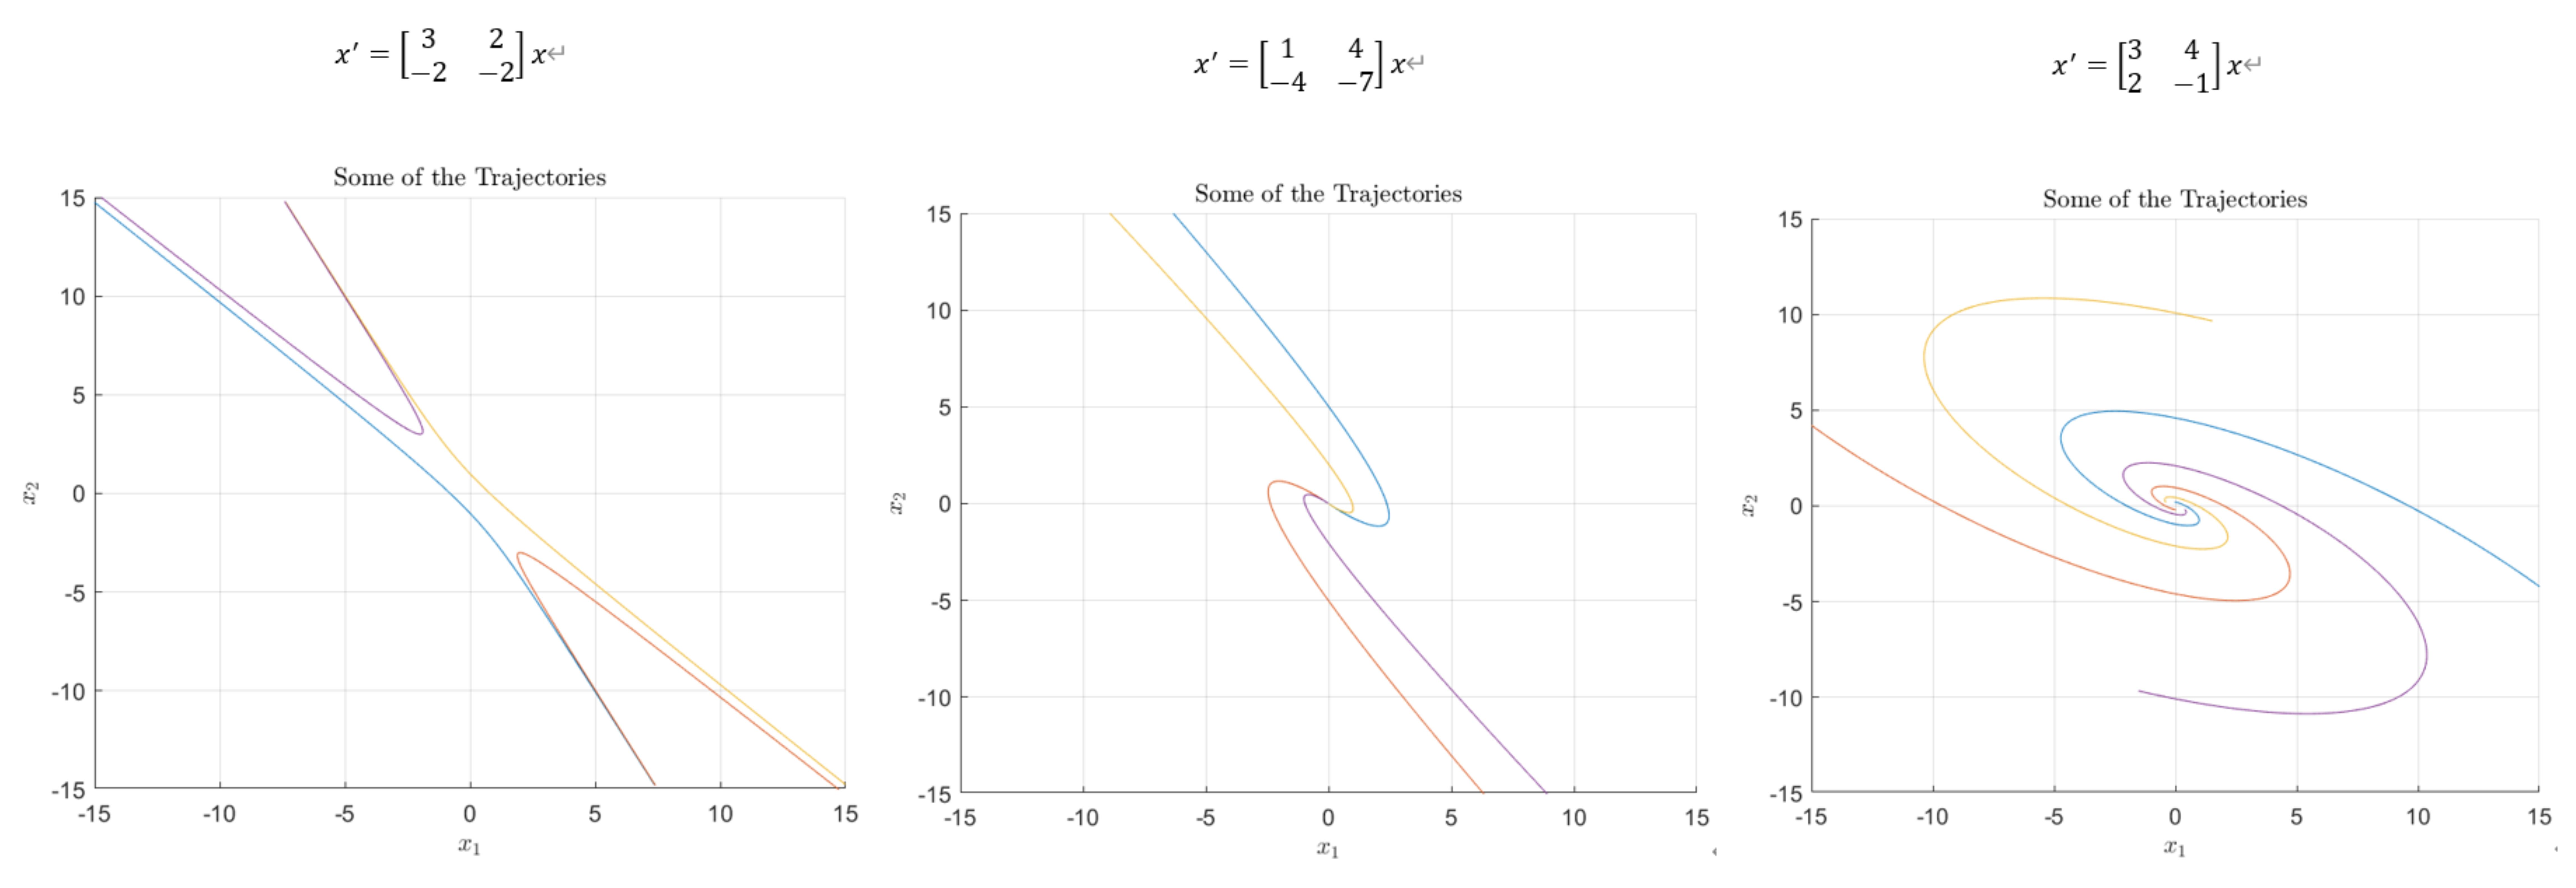
\includegraphics[width=\textwidth]{ode.jpg}
\end{figure}
If all the eigenvlues are negative, all the solution curve will go to the origin as time increases.
\end{frame}

\begin{frame}{Definition of Positive Definiteness}
We give 2 definitions here in different perspectives:
\begin{itemize}
    \item Algebra: All the eigenvalues corresponding to this matrix are positive.
    \item Geometry: $f\left( \mathbf{x} \right) =\mathbf{x}^TA\mathbf{x}>0$ for all nonzero real vector $x$.
\end{itemize}

What is $\mathbf{x}^TA\mathbf{x}$? Do matrix multiplication in 2-dimensional:
\begin{equation*}
    \mathbf{x}^TA\mathbf{x}=\left[ \begin{matrix}
        x_1&		x_2\\
    \end{matrix} \right] \left[ \begin{matrix}
        a&		b\\
        b&		c\\
    \end{matrix} \right] \left[ \begin{array}{c}
        x_1\\
        x_2\\
    \end{array} \right] ={ax_1}^2+2bx_1x_2+{cx_2}^2
\end{equation*}

Can you have a direct imagination of $\mathbf{x}^TA\mathbf{x}$? If the matrix $A$ is positive definite, it is like a bowl. Imagine the plane $\mathbf{x}^TA\mathbf{x}=1$, you can get an ellipse!

\vspace{3pt}
A website for fun: \url{https://www.wolframalpha.com/}

\vspace{3pt}
Try with example:
\begin{equation*}
    \mathbf{x}^TA\mathbf{x}=\left[ \begin{matrix}
        x_1&		x_2\\
    \end{matrix} \right] \left[ \begin{matrix}
        2&		2\\
        2&		5\\
    \end{matrix} \right] \left[ \begin{array}{c}
        x_1\\
        x_2\\
    \end{array} \right] =2{x_1}^2+4x_1x_2+5{x_2}^2
\end{equation*}
\end{frame}

\begin{frame}{Tests for Positive Definiteness}
    Tests for Positive Definiteness:
\begin{enumerate}
    \item $f\left( \mathbf{x} \right) =\mathbf{x}^TA\mathbf{x}>0$ for all nonzero real vector $x$.
    \item All the eigenvalues of $A$ satisfy $\lambda _i>0$.
    \item All the leading submatrices $A_k$ have positive determinants.
    \item All the pivots (without row exchanges) satisfy $d_k>0$.
\end{enumerate}

\vspace{3pt}
Test 2 and 4 are easy to understand, how about test 3? In my view, determinat combines pivots and eigenvalues together.

\vspace{3pt}
Although we have 4 tests, actually test 2, 3, 4 are showing the same thing.

\begin{equation*}
    \mathbf{x}^TA\mathbf{x}=\left[ \begin{matrix}
        x_1&		x_2\\
    \end{matrix} \right] \left[ \begin{matrix}
        2&		2\\
        2&		5\\
    \end{matrix} \right] \left[ \begin{array}{c}
        x_1\\
        x_2\\
    \end{array} \right] =2{x_1}^2+4x_1x_2+5{x_2}^2
\end{equation*}

Please use the four tests to show that matrix $A$ is positive definite. (You may need to verify the first test by completing the squares.)

\end{frame}

\begin{frame}{Tests for Positive Definiteness}
\begin{equation*}
    \mathbf{x}^TA\mathbf{x}=\left[ \begin{matrix}
        x_1&		x_2\\
    \end{matrix} \right] \left[ \begin{matrix}
        2&		2\\
        2&		5\\
    \end{matrix} \right] \left[ \begin{array}{c}
        x_1\\
        x_2\\
    \end{array} \right] =2{x_1}^2+4x_1x_2+5{x_2}^2
\end{equation*}
Let's start with test 2:
\begin{equation*}
    \det \left( A-\lambda I \right) =\left| \begin{matrix}
        2-\lambda&		2\\
        2&		5-\lambda\\
    \end{matrix} \right|=\left( \lambda -1 \right) \left( \lambda -6 \right) =0
\end{equation*}
Eigenvalues are $\lambda _1=1, \lambda _2=6$, all greater than zero.

\vspace{3pt}
Test 3:
\begin{equation*}
    |2|=2>0, \left| \begin{matrix}
        2&		2\\
        2&		5\\
    \end{matrix} \right|=6>0
\end{equation*}

\vspace{3pt}
Test 4:
\begin{equation*}
    \left[ \begin{matrix}
        2&		2\\
        2&		5\\
    \end{matrix} \right] \rightarrow \left[ \begin{matrix}
        {\color[RGB]{240, 0, 0} 2}&		2\\
        0&		{\color[RGB]{240, 0, 0} 3}\\
    \end{matrix} \right]
\end{equation*}
\end{frame}

\begin{frame}{Tests for Positive Definiteness}
    \begin{equation*}
    \mathbf{x}^TA\mathbf{x}=\left[ \begin{matrix}
        x_1&		x_2\\
    \end{matrix} \right] \left[ \begin{matrix}
        2&		2\\
        2&		5\\
    \end{matrix} \right] \left[ \begin{array}{c}
        x_1\\
        x_2\\
    \end{array} \right] =2{x_1}^2+4x_1x_2+5{x_2}^2
\end{equation*}
Finally, check with test 1. Typically, we finish this by completing the squares.
\begin{equation*}
    2{x_1}^2+4x_1x_2+5{x_2}^2=2{x_1}^2+4x_1x_2+2{x_2}^2+3{x_2}^2=2\left( x_1+x_2 \right) ^2+3{x_2}^2>0
\end{equation*}

This is a simple example, but in most of the cases, we cannot complete the squares by observation. There is actually a linear algebra way to do this! Recall your knowledge of $LDL^T$ factorization.

\begin{equation*}
    \left[ \begin{matrix}
        2&		2\\
        2&		5\\
    \end{matrix} \right] =\left[ \begin{matrix}
        1&		0\\
        1&		1\\
    \end{matrix} \right] \left[ \begin{matrix}
        2&		2\\
        0&		3\\
    \end{matrix} \right] \left[ \begin{matrix}
        1&		1\\
        0&		1\\
    \end{matrix} \right]
\end{equation*}

Can observe that $LDL^T$ can guide you how to complete the squares. Why?
\end{frame}

\begin{frame}{Linear Algebra Way for Completing Squares}
    \begin{equation*}
        2{x_1}^2+4x_1x_2+5{x_2}^2=2\left( x_1+x_2 \right) ^2+3{x_2}^2>0
    \end{equation*}
    \begin{equation*}
        \left[ \begin{matrix}
            2&		2\\
            2&		5\\
        \end{matrix} \right] =\left[ \begin{matrix}
            1&		0\\
            1&		1\\
        \end{matrix} \right] \left[ \begin{matrix}
            2&		2\\
            0&		3\\
        \end{matrix} \right] \left[ \begin{matrix}
            1&		1\\
            0&		1\\
        \end{matrix} \right]
    \end{equation*}
Change $A=LDL^T$ in:
\begin{equation*}
    x^TAx=x^TLDL^Tx=\left( L^Tx \right) ^TD\left( L^Tx \right)
\end{equation*}

\vspace{3pt}
Adopt change of variable $y=L^Tx$:
\begin{equation*}
    \left[ \begin{array}{c}
        y_1\\
        y_2\\
    \end{array} \right] =\left[ \begin{matrix}
        1&		1\\
        0&		1\\
    \end{matrix} \right] \left[ \begin{array}{c}
        x_1\\
        x_2\\
    \end{array} \right] , \begin{cases}
        y_1=x_1+x_2\\
        y_2=x_2\\
    \end{cases}
\end{equation*}
\begin{equation*}
    x^TAx=y ^TDy
\end{equation*}
The pivots are the coefficients of the squares. In this example, 2 and 3.
\end{frame}

\begin{frame}{Linear Algebra Way for Completing Squares}
    You also have $A=Q\varLambda Q^T$ factorization!

    \vspace{3pt}
    Change $A=Q\varLambda Q^T$ in:
\begin{equation*}
    x^TAx=x^TQ\varLambda Q^Tx=\left( Q^Tx \right) ^TD\left( Q^Tx \right)
\end{equation*}

Let's have a try!
\begin{equation*}
    \left[ \begin{matrix}
        2&		2\\
        2&		5\\
    \end{matrix} \right] =\left[ \begin{matrix}
        \frac{2}{\sqrt{5}}&		\frac{1}{\sqrt{5}}\\
        \frac{-1}{\sqrt{5}}&		\frac{2}{\sqrt{5}}\\
    \end{matrix} \right] \left[ \begin{matrix}
        1&		0\\
        0&		6\\
    \end{matrix} \right] \left[ \begin{matrix}
        \frac{2}{\sqrt{5}}&		\frac{-1}{\sqrt{5}}\\
        \frac{1}{\sqrt{5}}&		\frac{2}{\sqrt{5}}\\
    \end{matrix} \right]
\end{equation*}
\begin{equation*}
    \left[ \begin{array}{c}
        y_1\\
        y_2\\
    \end{array} \right] =\left[ \begin{matrix}
        \frac{2}{\sqrt{5}}&		\frac{-1}{\sqrt{5}}\\
        \frac{1}{\sqrt{5}}&		\frac{2}{\sqrt{5}}\\
    \end{matrix} \right] \left[ \begin{array}{c}
        x_1\\
        x_2\\
    \end{array} \right] , \begin{cases}
        y_1=\frac{2}{\sqrt{5}}x_1-\frac{1}{\sqrt{5}}x_2\\
        y_2=\frac{1}{\sqrt{5}}x_1+\frac{2}{\sqrt{5}}x_2\\
    \end{cases}
\end{equation*}
\begin{equation*}
    2{x_1}^2+4x_1x_2+5{x_2}^2=\left( \frac{2}{\sqrt{5}}x_1-\frac{1}{\sqrt{5}}x_2 \right) ^2+6\left( \frac{1}{\sqrt{5}}x_1+\frac{2}{\sqrt{5}}x_2 \right) ^2>0
\end{equation*}

Note that not all real symmetric matrices can have $A=LU$ factorization, but they must have $A=Q\varLambda Q^T$ factorization.

\end{frame}

\begin{frame}{The Principle Axes Theorem}
Here is the chapter 6 meaning of $A=Q\varLambda Q^T$ factorization. I will use the knowledge in senior high school to show you.

\vspace{3pt}
Use the example in the slide above.
\begin{equation*}
    2{x_1}^2+4x_1x_2+5{x_2}^2=\left( \frac{2}{\sqrt{5}}x_1-\frac{1}{\sqrt{5}}x_2 \right) ^2+6\left( \frac{1}{\sqrt{5}}x_1+\frac{2}{\sqrt{5}}x_2 \right) ^2>0
\end{equation*}

Change of variable and let the quadratic form equals 1:
\begin{equation*}
    \begin{cases}
        y_1=\frac{2}{\sqrt{5}}x_1-\frac{1}{\sqrt{5}}x_2\\
        y_2=\frac{1}{\sqrt{5}}x_1+\frac{2}{\sqrt{5}}x_2\\
    \end{cases}
\end{equation*}
\begin{equation*}
    2{x_1}^2+4x_1x_2+5{x_2}^2={y_1}^2+6{y_2}^2=1
\end{equation*}

That is the equation of an ellipse! Imagine in your mind: the shape at height 1 is a ellipse. And the change of varible is like rotating the axes, which lands on the axes on the ellipse.
\end{frame}

\begin{frame}{Congruence Transformation}
\begin{definition}
    For an invertible matrix $C$, the linear transformation $A\mapsto C^TAC$ is called a congruence transformation.
\end{definition}

Essence: change of variable $x$ to $y$ and the quadratic form remains unchanged.

\vspace{3pt}
The symmetry, rank, signs of eigenvalues are all hold before and after the transformation. That is because, the quadratic form behind never change.

\vspace{3pt}
Recall another transformation we meet in 5.6: similarity transformation $B=M^{-1}AM$. Which variables are not changed?
\end{frame}

\begin{frame}{Transform to Standard Quadratic Form}
We have introduced 2 approaches: $A=LDL^T$ factorization and $A=Q\varLambda Q^T$ factorization. Here we use another method: Elementary Transformation.

\begin{equation*}
    f\left( x_1, x_2, x_3 \right) ={x_1}^2+2{x_2}^2+5{x_3}^2+2x_1x_2+2x_1x_3+6x_2x_3
\end{equation*}
\begin{equation*}
    \left[ \begin{array}{c}
        A\\
        I\\
    \end{array} \right] =\left[ \begin{matrix}
        1&		1&		1\\
        1&		2&		3\\
        1&		3&		5\\
        1&		0&		0\\
        0&		1&		0\\
        0&		0&		1\\
    \end{matrix} \right] \rightarrow \left[ \begin{matrix}
        1&		0&		0\\
        0&		1&		2\\
        0&		2&		4\\
        1&		-1&		-1\\
        0&		1&		0\\
        0&		0&		1\\
    \end{matrix} \right] \rightarrow \left[ \begin{matrix}
        1&		0&		0\\
        0&		1&		0\\
        0&		0&		0\\
        1&		-1&		1\\
        0&		1&		-2\\
        0&		0&		1\\
    \end{matrix} \right] =\left[ \begin{array}{c}
        D\\
        C\\
    \end{array} \right]
\end{equation*}

Change of variable: $x=Cy$, then it will be standard quadratic form.

\vspace{3pt}
The key: do symmtric row and colomn operations for $A$, and only do column operations for $I$.

\vspace{3pt}
My suggestion: $A=LDL^T$ factorization is yyds!
\end{frame}

\section{Singular Value Decomposition}
\begin{frame}{Introduction}
We have introduced so many different decomposition for square matrices in Chapter 5, but what about non-square matrices?

All decomposition for non-square matrices:
\begin{enumerate}
    \item $PA=LU$, $P$ is permutation matrix, $L$ is lower triangular matrix with 1s on the diagonal, and $U$ is the "upper something", echelon form.
    \item $A=QR$, $Q$ is matrix with orthonormal columns, $R$ is an upper triangular matrices.
\end{enumerate}

Here we have the third one: singular value decomposition $A=U\varSigma V^T$.

\vspace{3pt}
Try to guess the size and properties of these 3 matrices.
\end{frame}
\end{document}